\subsection{Geometry}

The simulation of the \gluex DIRC detector within the \gluex software is based on {\geant}4 (\texttt{hdgeant4} package). The \gluex DIRC in simulation is defined by the geometry description (located in  \texttt{hdds/DIRC{\_}HDDS.xml}) and the functionality of the sensitive elements (described in \texttt{hdgeant4/src/GlueXSensitiveDetectorDIRC} class). 

The detector geometry is an important part of the detector simulation. It should represent all main features of the detector and contain all the elements responsible for the detector response. At the same time it should be simple and contain as few geometrical constituents as possible to keep the simulation fast. The \gluex DIRC geometry is shown in Fig.~\ref{pic:dirc}. Each volume is defined by its shape and material (the list of materials for the \gluex simulation is in \texttt{hdds/Material{\_}HDDS.xml}). 

\begin{figure}[!h]
\centering
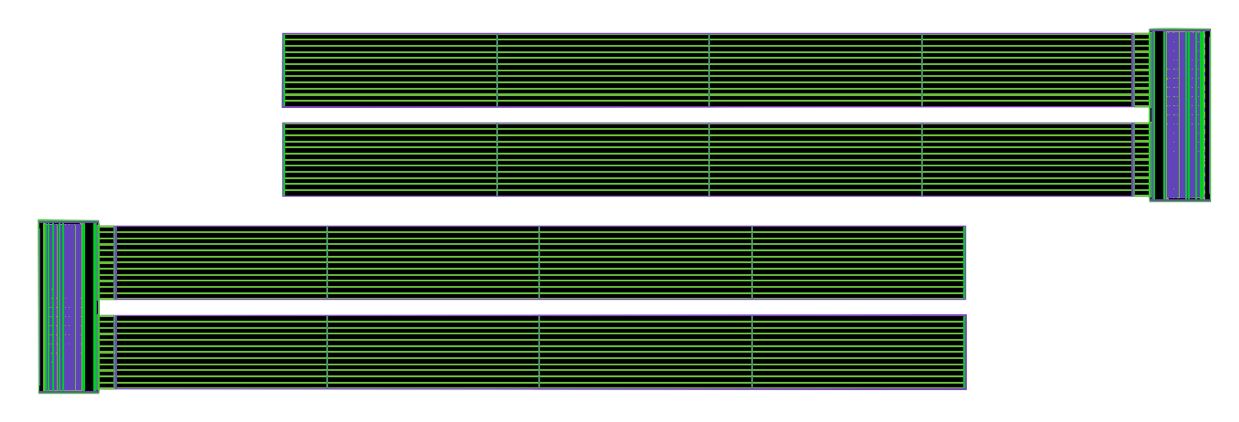
\includegraphics[width=0.8\textwidth]{pics/bars1.png}\\
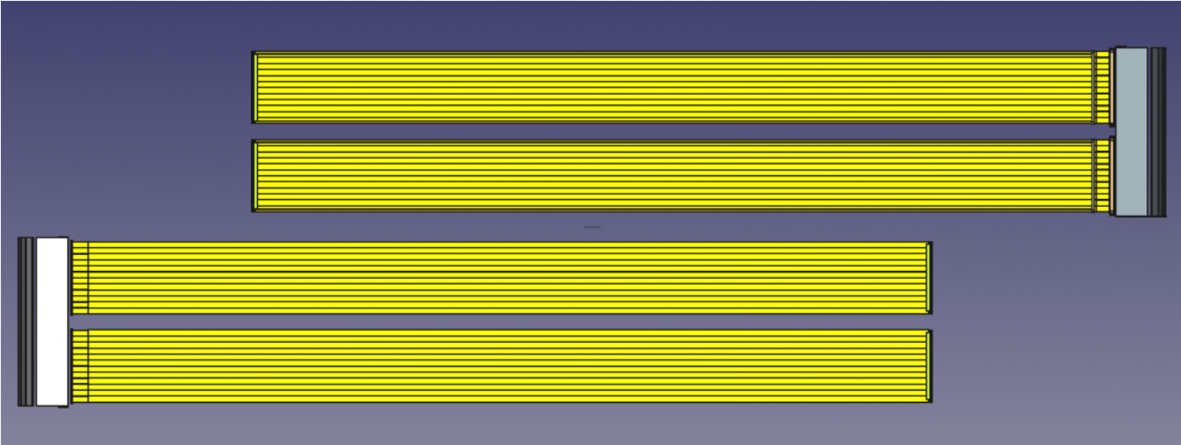
\includegraphics[width=0.8\textwidth]{pics/bars2.png}
\caption{\label{pic:dirc}
Simulation (top) and CAD drawings (bottom) of the \gluex DIRC.
}
\end{figure}  

\begin{figure}[!h]
\centering
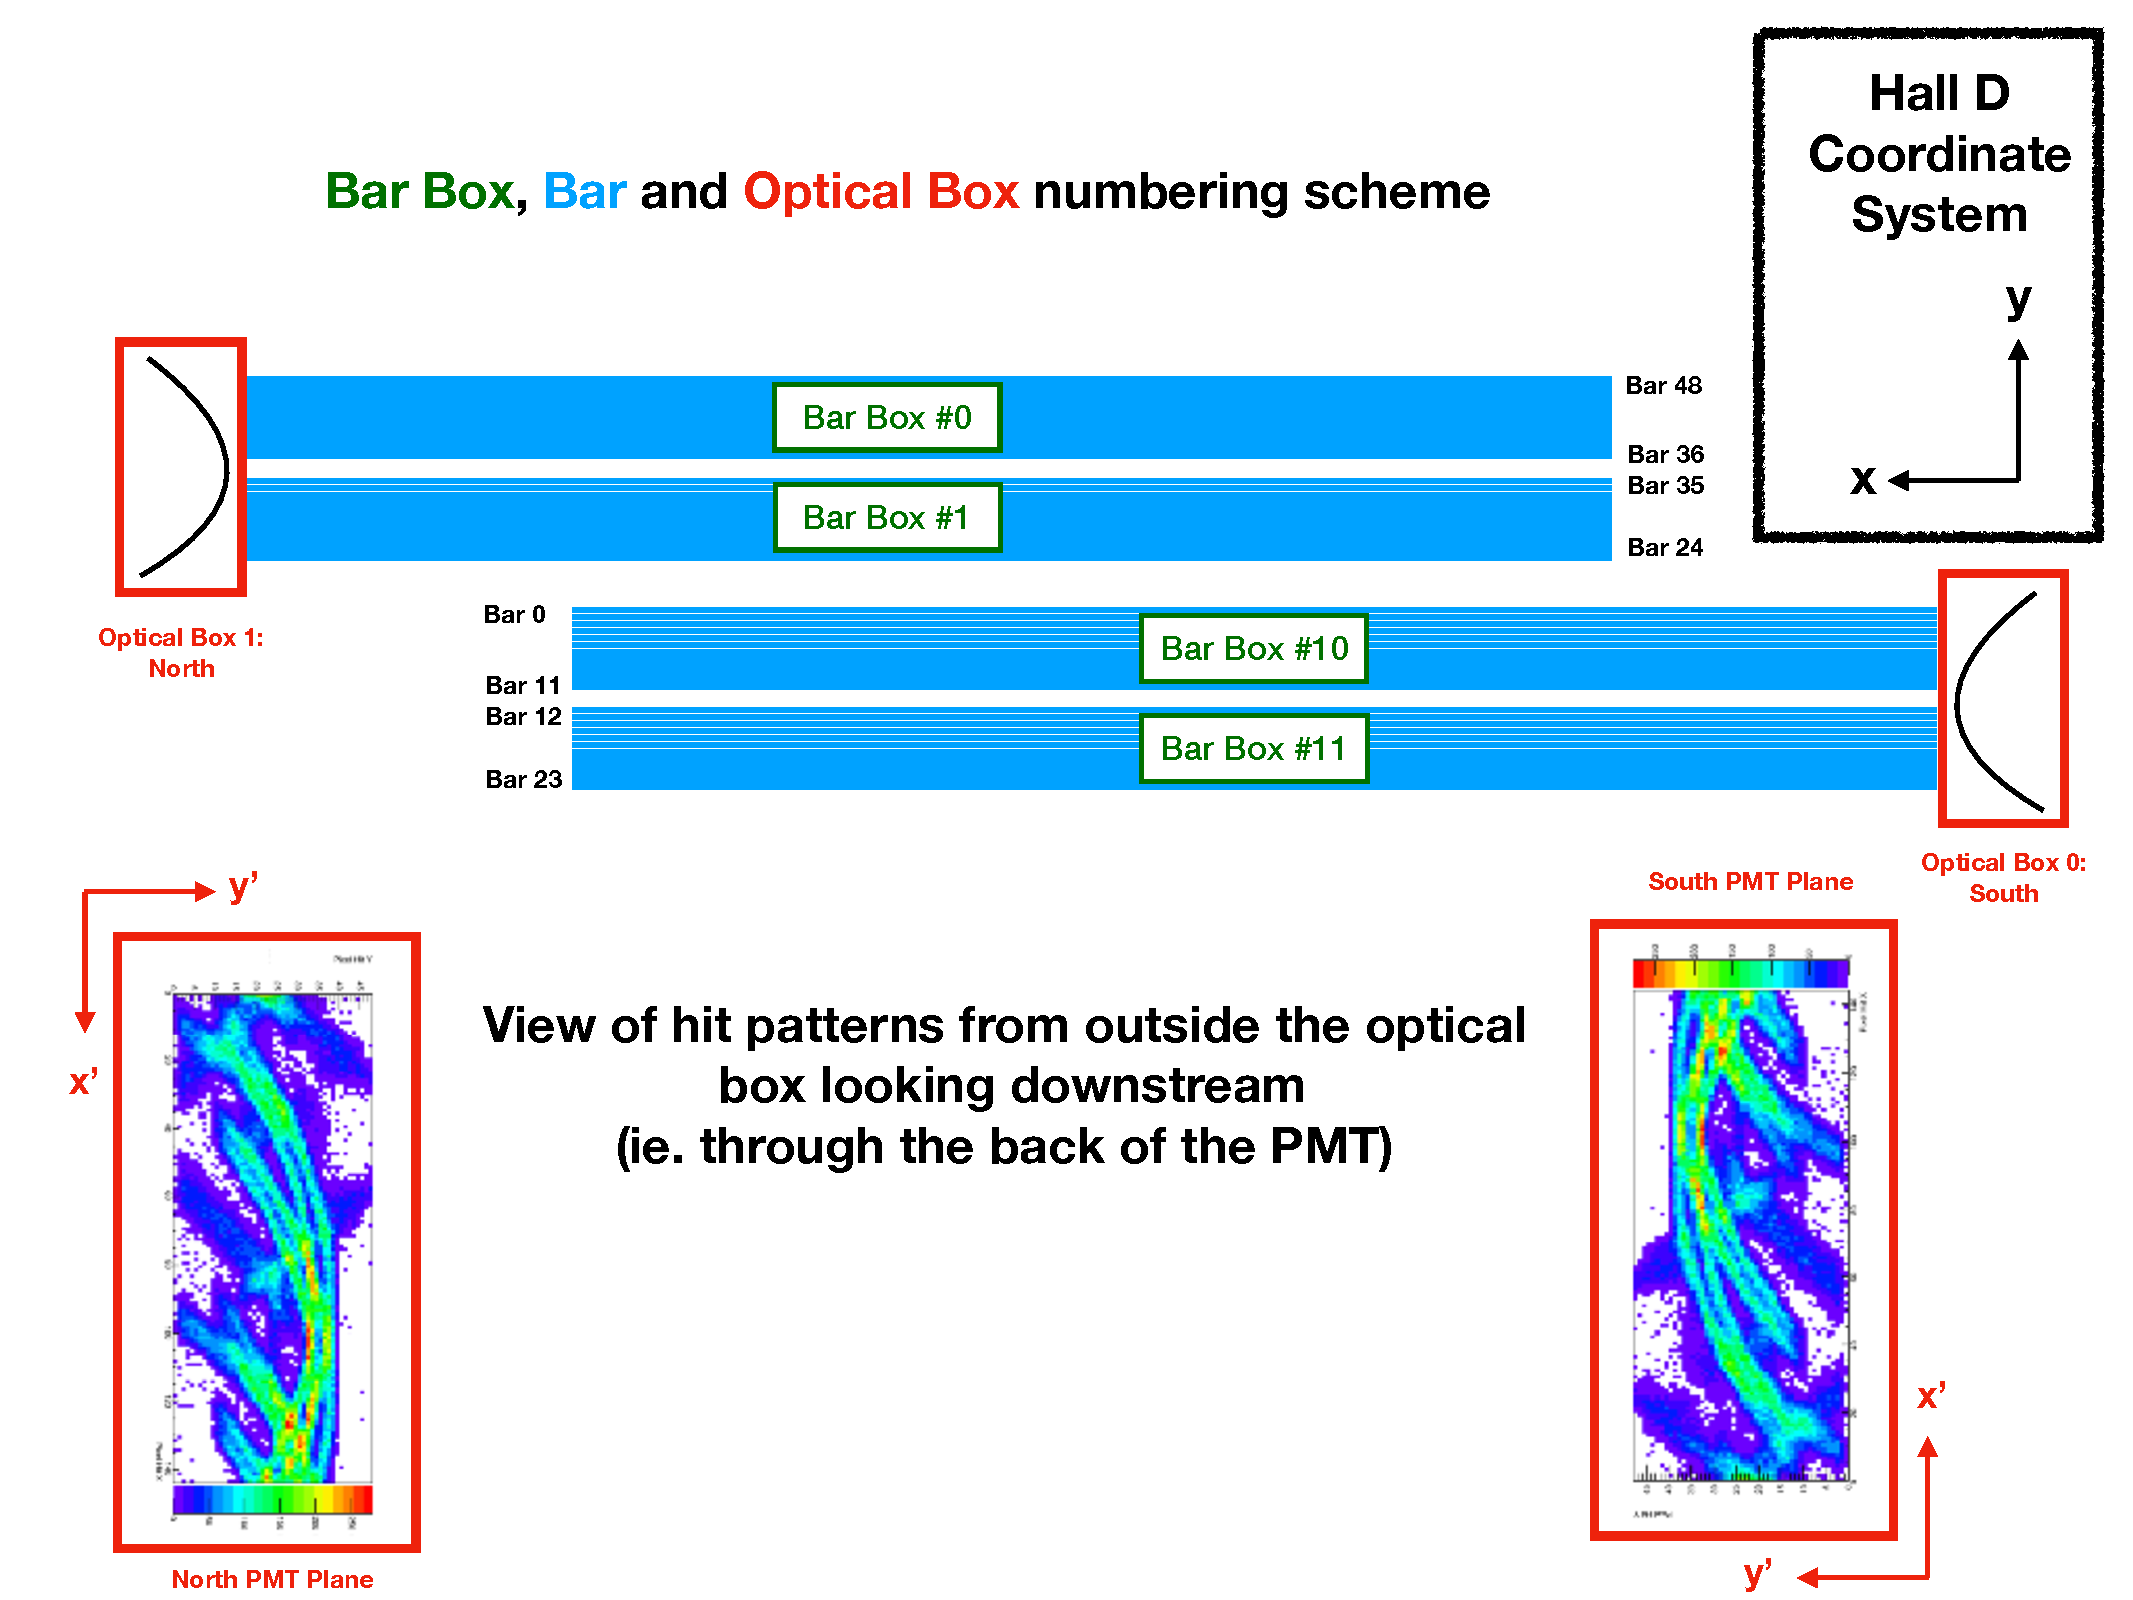
\includegraphics[width=0.98\textwidth]{pics/DIRC_Geometry11.pdf}\\
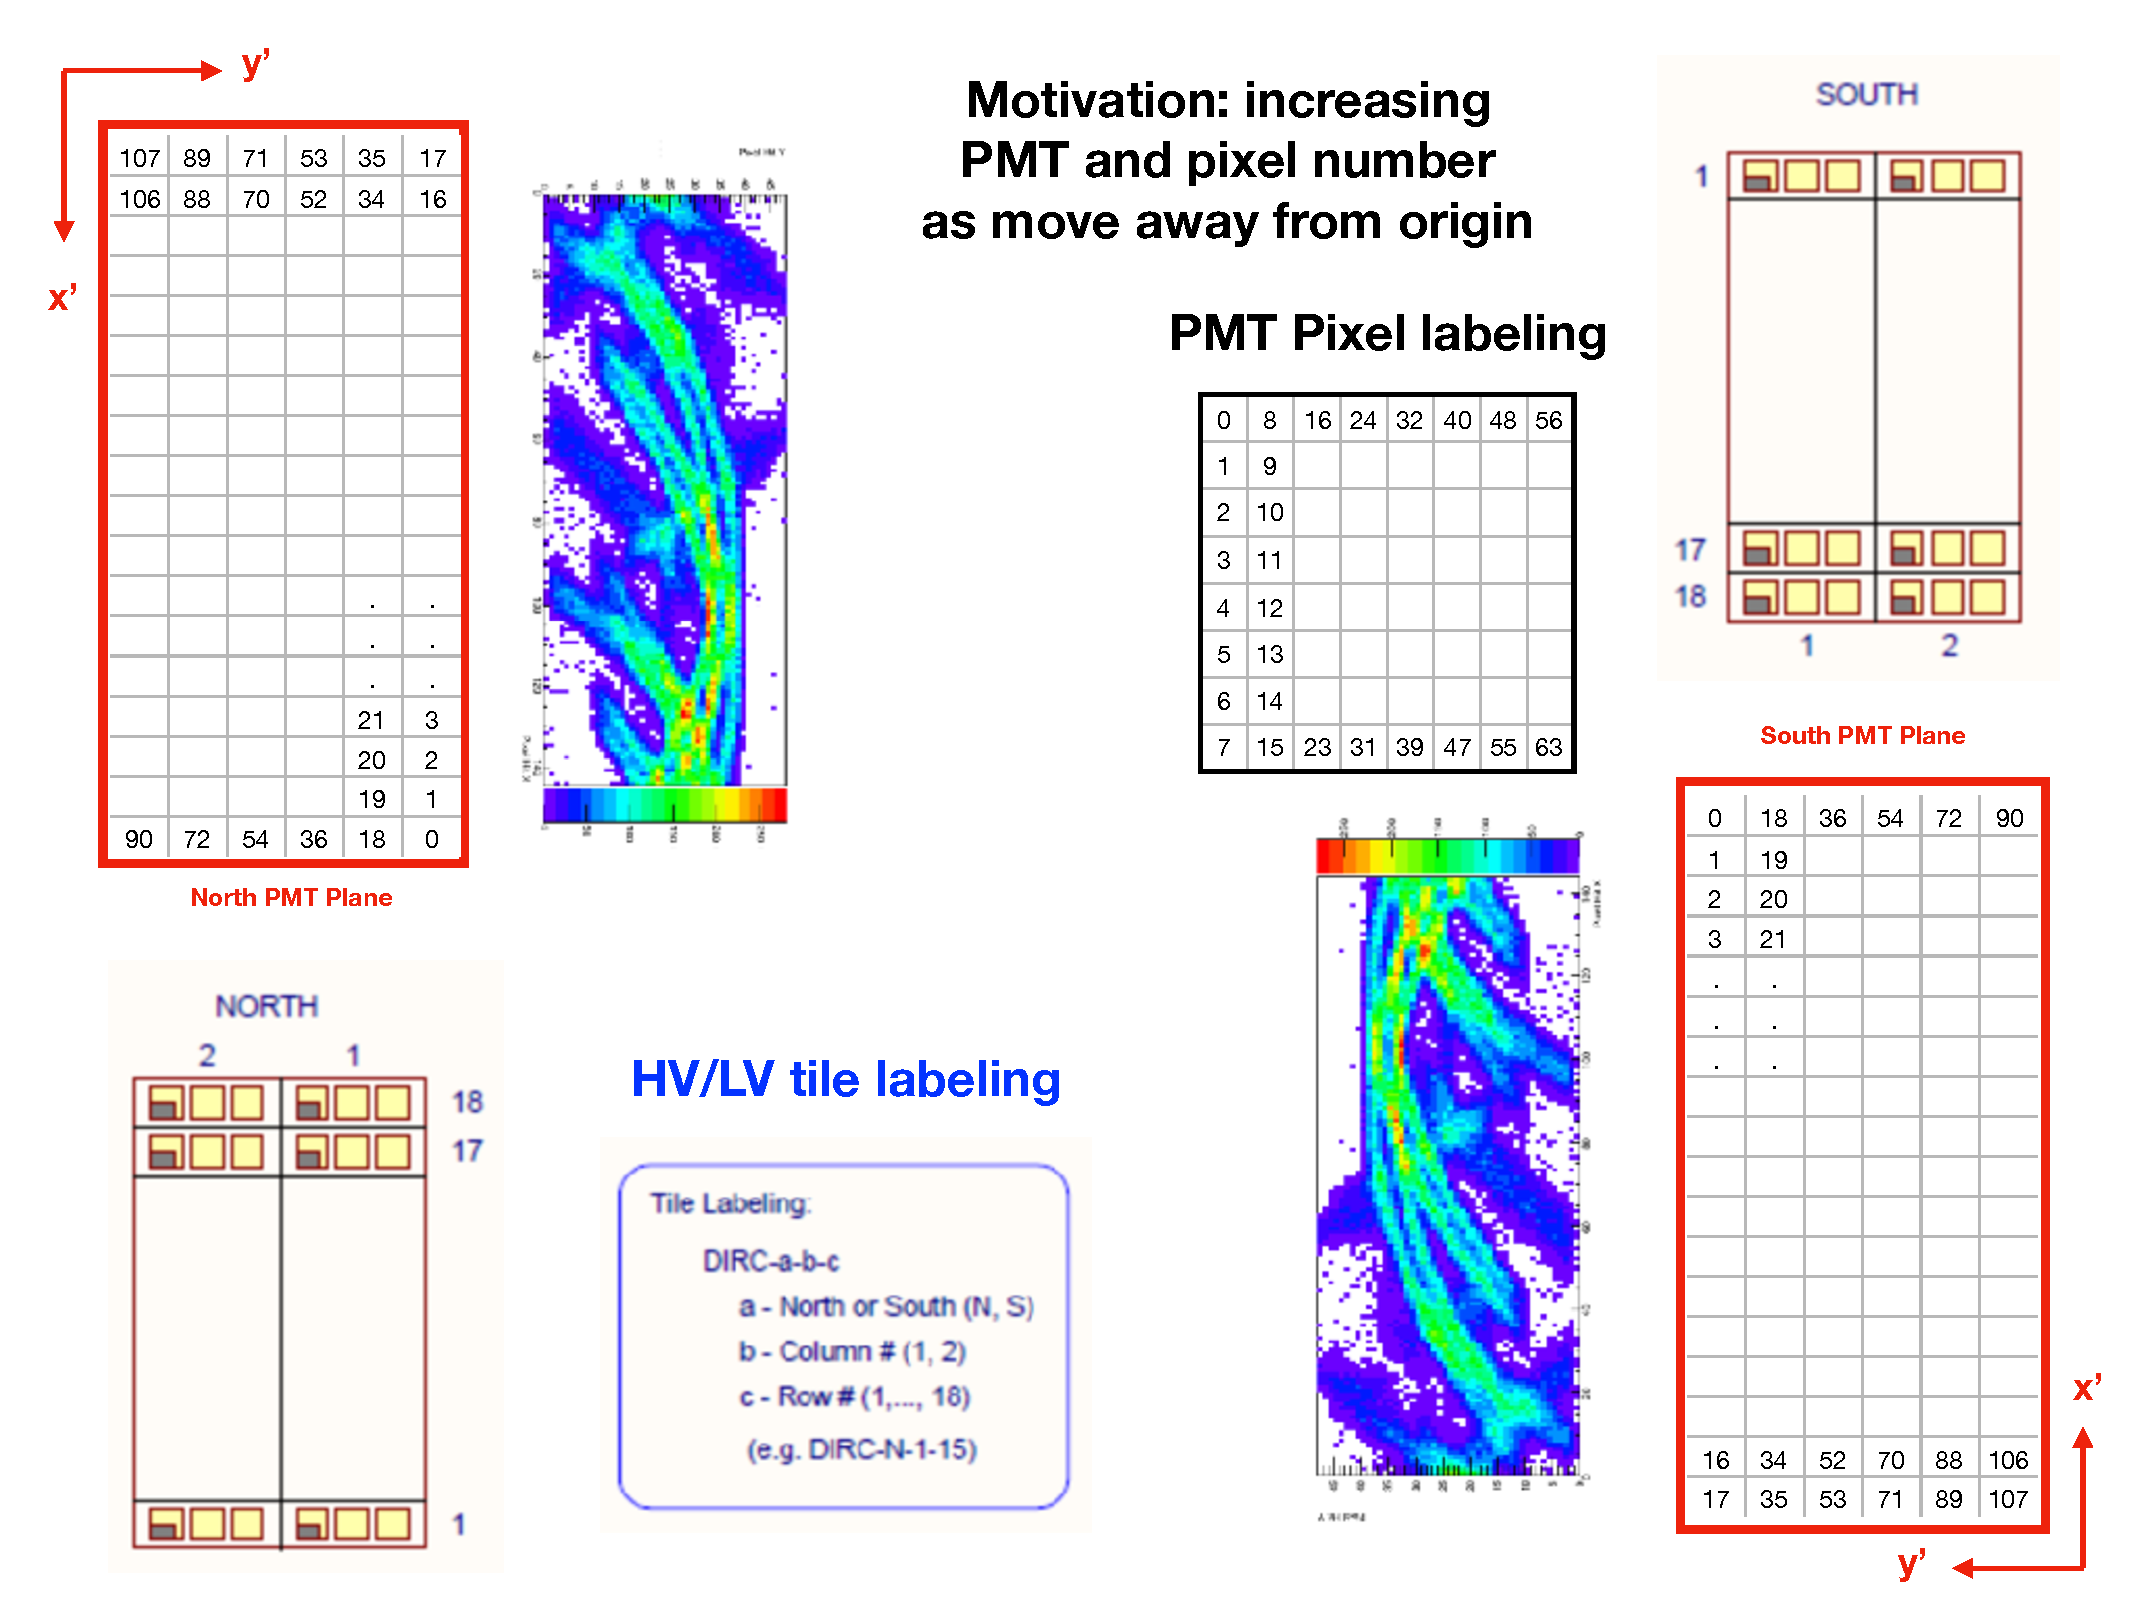
\includegraphics[width=0.98\textwidth]{pics/DIRC_Geometry22.pdf}
\caption{\label{pic:dirc2}
Numbering schemes of the DIRC constituents.
}
\end{figure}

\vspace{0.5cm}
Some basic rules for constructing a \geant geometry:
\begin{itemize}
\item \geant supports hierarchy, when daughter-volumes are located inside of a mother-volume.  Here one should make sure the daughter-volumes are completely within the mother volume. In case some part of a daughter-volume sticks out from the mother volume, a so-called ``overlap'' occurs. Such overlaps should be avoided. To check for overlaps, one has to uncomment the line \texttt{CHECK{\_}OVERLAPS{\_}MM} in the \texttt{GNUmakefile} in the top directory of the \texttt{hdgeant4} project and then recompile the \texttt{hdgeant4} project (for this do \texttt{touch src/HddsG4Builder.cc} and then \texttt{make} -- this only rebuilds classes that need to change)
\item The coordinates of the daughter-volume are set in the local coordinate system of the mother volume. The origin is at the center of the mother volume, if it is a box, and should be looked up in the {\geant}4 manuals otherwise
\item When creating a volume, e.g.
%\vspace{0.5cm}
\begin{center}
 \texttt{<box name="DCMV" X{\_}Y{\_}Z="560.0 250.0 150.0" material="OpticalAir" />} 
\end{center}
%\vspace{0.5cm}
\noindent its full (not half) dimenstions should be set. Here the box has dimensions of 560 cm x 250 cm x 150 cm.
\item Volumes can be grouped in assemblies called compositions. Inside a composition volumes are located with respect to the center of the composition. When the composition is placed inside the mother-volume, its center is placed with respect to the center of the mother-volume.
\end{itemize}

The DIRC can be activated or deactivated by commenting in/out the corresponding line in the \texttt{main{\_}HDDS.xml} file (lines 82-83): 

\vspace{0.5cm}
\begin{center}
 \texttt{<!- - To simulate DIRC hits uncomment the line below - -> \\
    <!- -posXYZ volume="DIRC" X{\_}Y{\_}Z="0.0 0.0 595.0" /- ->} 
\end{center}
\label{eq:line}
\vspace{0.5cm}

The \texttt{DIRC} object, which is placed inside the virtual Hall D when the line above is active, is an auxiliary volume in a shape of a rectangular block containing the DIRC detector (see Fig.~\ref{pic:sim}). Its coordinates are defined in the global coordinate system of the hall, in which the $z$ axis goes along the beam, $x$ axis is parallel to the floor, and the $y$ axis is vertical. The target center is at $(0, 0, 65)$ cm. The center of the \texttt{DIRC} volume is at $z = 595$ cm.
Taking into account the z locations of the daughter volumes \texttt{DRCC} (composition holding the DIRC constituents), \texttt{DCML} (bar box), and \texttt{DCBR} (the radiator bar), the center of the radiator bar is currently at $z = 595 - 40 + 30 =585$ cm downstream the global 0. The distance from the center of the target ($(0, 0, 65)$ cm) is $585 - 65 = 520$ cm. The numbering schemes of individual volumes are represented in Fig.~\ref{pic:dirc2}.

\begin{figure}[!h]
\centering
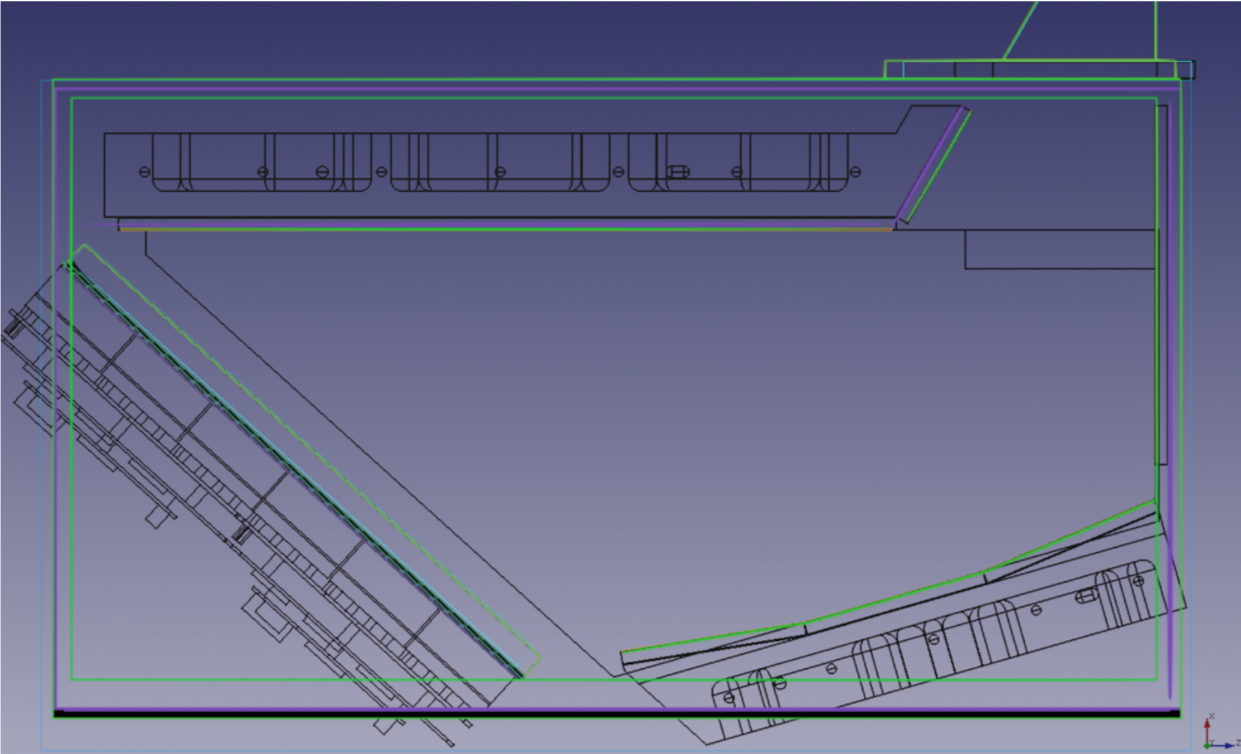
\includegraphics[width=0.8\textwidth]{pics/obgeom.png}
\caption{\label{pic:obg}
Geometry of the optical box overlayed with the CAD drawings illustrating the same locations of the mirrors. The optical elements are shown in green for the simulation and in black for the technical drawings.
}
\end{figure}

Realistic transport of Cherenkov photons through the optical elements of the detector from production to detection is essential for the DIRC simulation. Figures~\ref{pic:dirc} and~\ref{pic:obg} show that the current detector geometry matches the CAD technical drawings.

\begin{figure}[!htb]
\centering
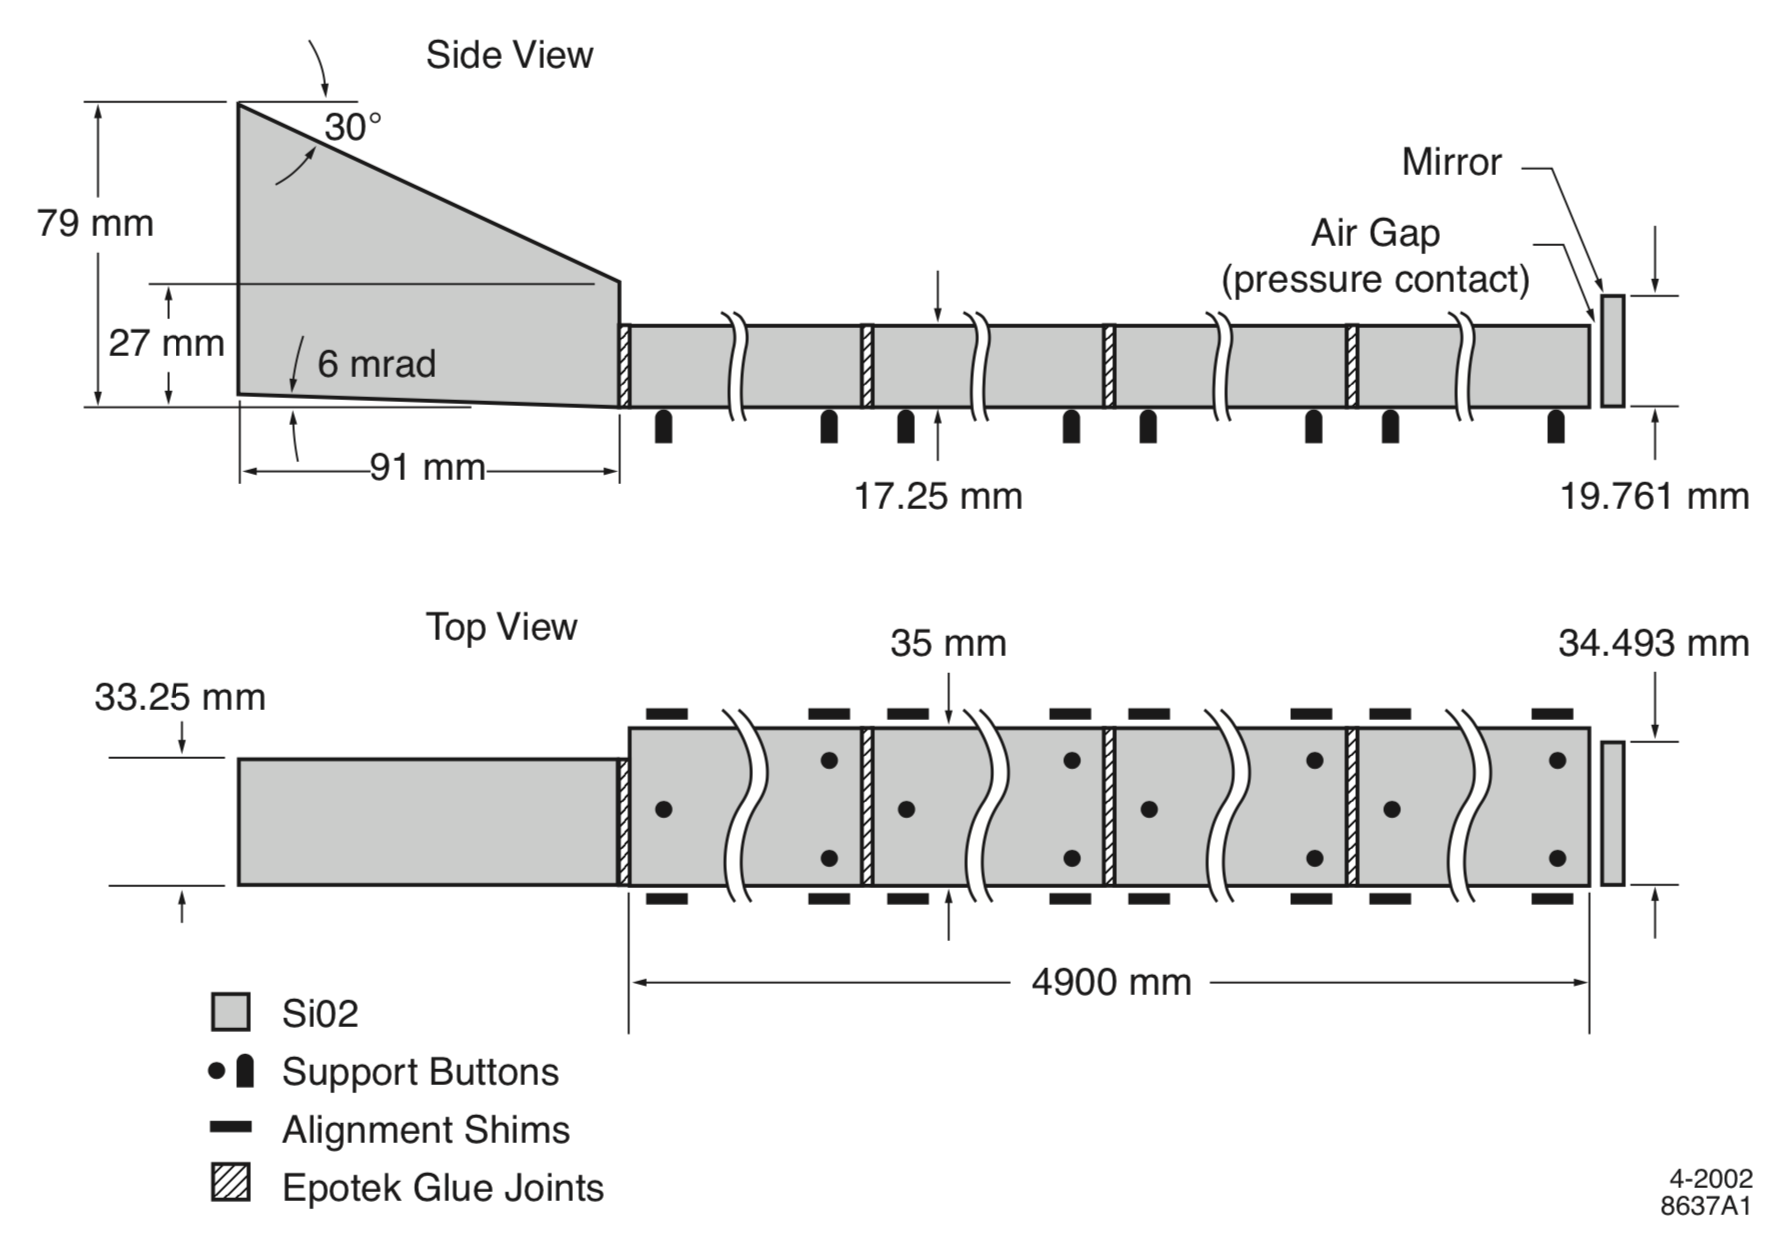
\includegraphics[width=0.8\textwidth]{pics/bars.png}
\caption{\label{pic:bar}
Schematic of the DIRC radiator bar in side and top view.
}
\end{figure} 

The structure of the radiator bar is shown in Fig.~\ref{pic:bar}. The mirror at the end of the bar has pressure contact with the fused silica bar, which implies an air gap. In simulation there is an air gap of $0.1$ mm between the mirror and the radiator bar. The schematic of the \gluex DIRC functional optical elements, illustrating different materials used in the simulation, is shown in Fig.~\ref{pic:struct}. 
The average bar dimensions are $35 \times 17.25 \times 4900 $ mm$^3$. The real measured bar sizes are being implemented into the geometry. 
\textcolor{red}{Here about the reaslistic bar size and locations! What is the spread of values? Reasons for implementing the measured values rather than average?...}Yunjie is working on this :) 

\begin{figure}[!h]
\centering
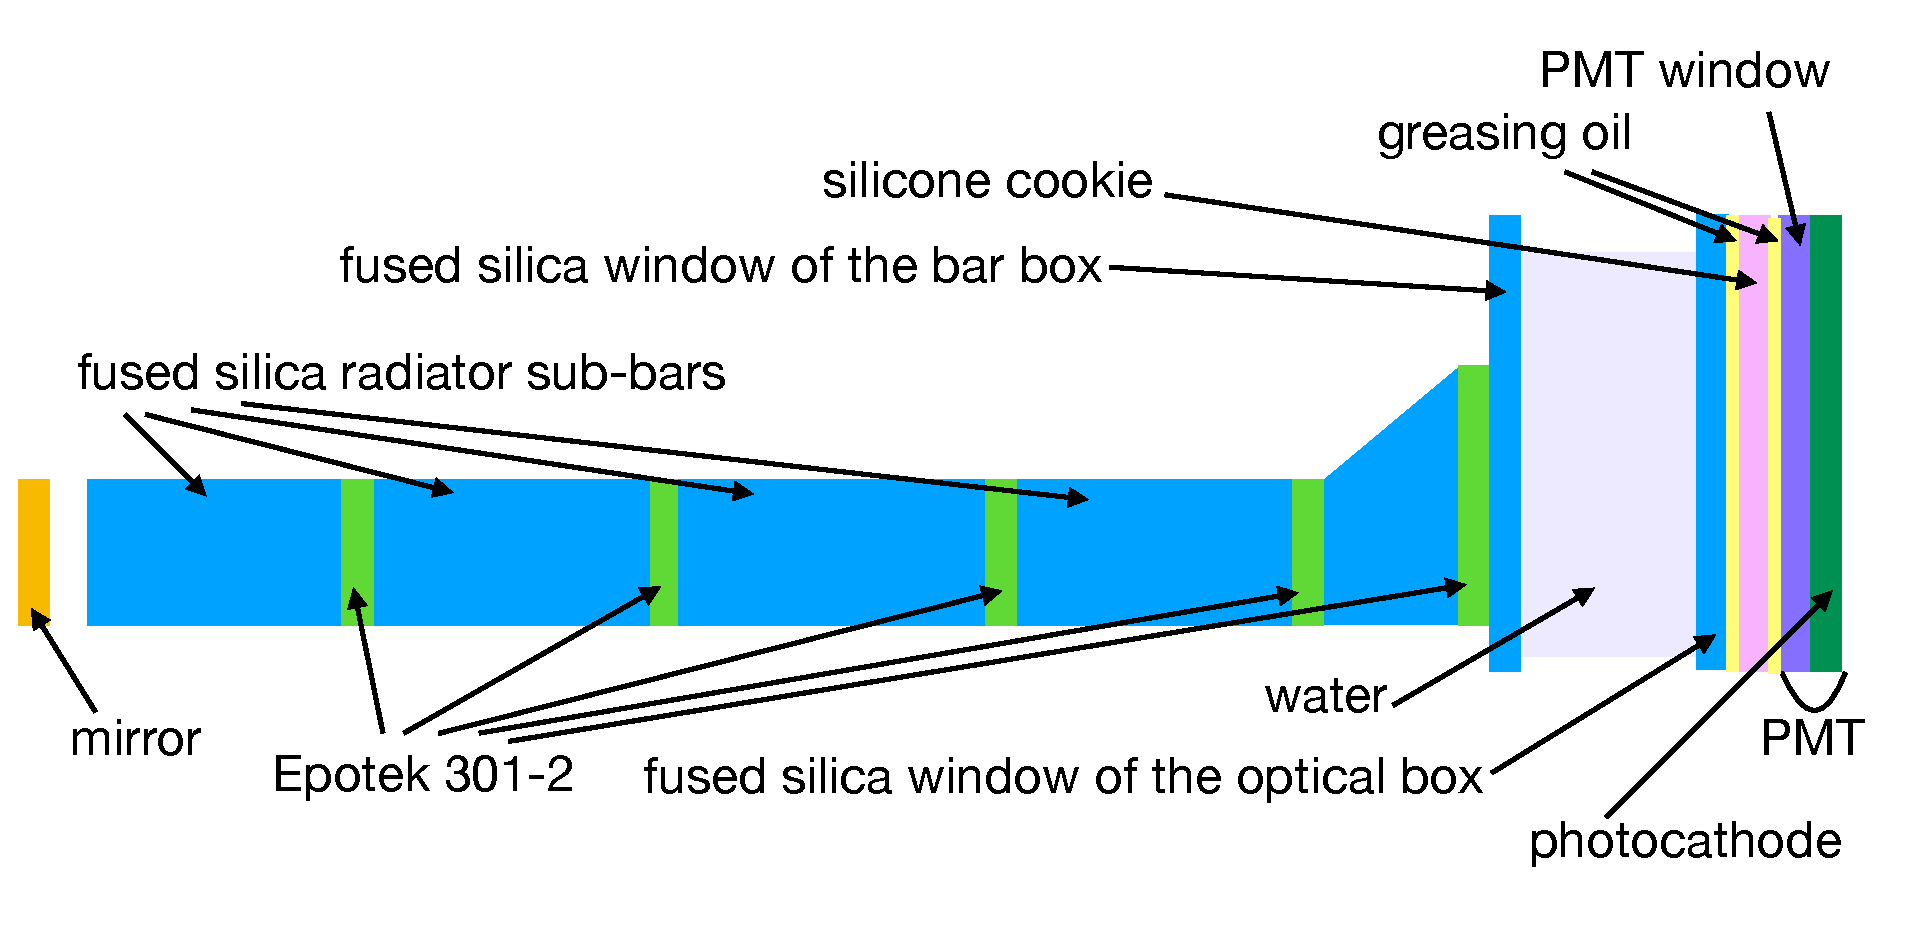
\includegraphics[angle=0,width=0.9\textwidth]{pics/struct3.pdf}
\caption{\label{pic:struct}
Schematic of one bar box in projection along the radiator length showing all the materials used for the optical system. Mirrors inside the optical box are omitted. The components are shown not to scale.
}
\end{figure}

The photosensors are implemented in a simplified way. One MaPMT is basically a stack of two layers: a borosilicate window and a bialkali photocathode, so that photons sequentially propagate through them (see Fig.~\ref{pic:struct}). The bialkali photocathode is set as a sensitive material for \geant 4, which means, that when a photon enters this volume, a special function is called, which writes out the detector signal. The functionality of the sensitive elements of the \gluex DIRC is described in \texttt{GlueXSensitiveDetectorDIRC} class.

The support structures located in the acceptance of the DIRC (shown in Fig.~\ref{pic:sim} as purple bars) are included in the simulation. They ensure proper material budget in front of the forward calorimeter.
